\section{Durchführung}
\label{sec:Durchführung}
Der Aufbau der Apparatur ist in Abbildung \ref{fig:aufbau} schematisch dargestellt.
\begin{figure}[H]
  \centering
  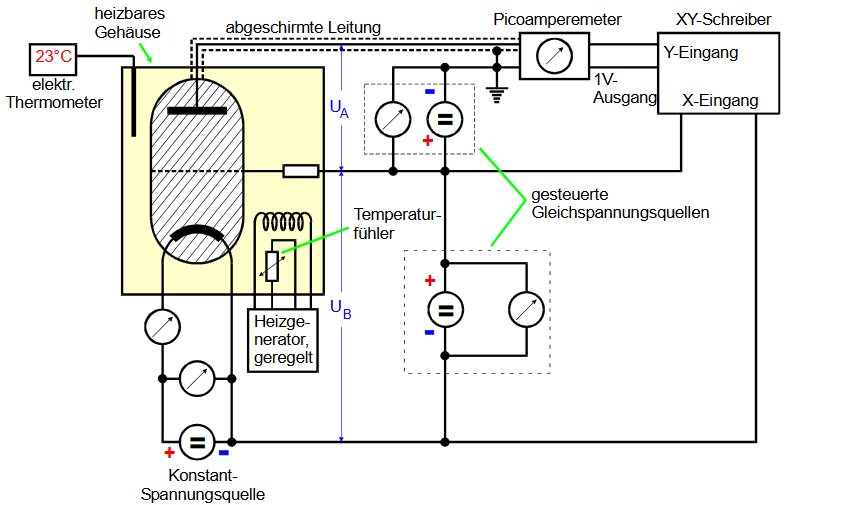
\includegraphics[width=\textwidth]{content/Aufbau.png}
  \caption{Aufbau des Versuchs\cite{v601}.}
  \label{fig:aufbau}
\end{figure}
\noindent Dieser besteht im Wesentlichen aus einem evakuiertem Gefäß.
In dem Gefäß befindet sich Hg-Dampf, Beschleunigerelektrode, Auffängerelektrode und Glühdraht.
Der Dampfdruck kann über einen Heizgenerator reguliert und die Innentemperatur über ein elektrisches Thermometer ausgelesen werden.
An die Auffängerelektrode ist ein Picoamperemeter angeschlossen.
An den Aufbau kann ein $XY$-Schreiber angeschlossen werden
\subsection{Energieverteilung der beschleunigten Elektronen}
\label{sec:ene}
Die Beschleunigerspannung wird auf konstante $U_B=\SI{+11}{\volt}$ eingestellt.
Die Temperatur wird auf ungefähr $\SI{20}{\degreeCelsius}$ gehalten.
Die Bremsspannung wird an den $X$-Eingang angeschlossen und die Auffängerstrom auf den $Y$-Eingang.
Die $X$-Achse des $XY$-Schreibers wird so geeicht, dass die Maximalspannung der Messung eine volle Auslenkung in $X$-Richtung erzielt.
Der Auffängerstrom $I_A$ wird in Abhängigkeit der Bremsspannung $U_A$ gemessen.
Dafür wird ein Diagramm mit dem $XY$-Schreiber erstellt.
Der Messung wird für eine Temperatur zwischen $T=\SI{140}{\degreeCelsius}$ und $T=\SI{160}{\degreeCelsius}$ wiederholt.
\subsection{Aufnahme von Franck-Hertz-Kurven}
Die Bremsspannung wird auf $U_A = \SI{1}{\volt}$ eingestellt.
Die Beschleunigerspannung wird an den $X$-Eingang angeschlossen und die Auffängerstrom auf den $Y$-Eingang.
Die Messung wird für einen Bereich von $0 < U_B < 60\si{\volt}$ durchgeführt.
Die $X$-Achse wird wie in Kapitel \ref{sec:ene} beschrieben geeicht.
Es werden Frank-Hertz-Kurven für die Temperaturen $T_1= 170\si{\degreeCelsius}$, $T_2= 180\si{\degreeCelsius}$ und $T_3= 190\si{\degreeCelsius}$ aufgezeichnet.
Die Kurve mit den am besten ersichtlichen Maximas wird ein weiteres mal in ein neues Diagramm eingezeichnet.
\subsection{Ionisierungsspannung von Hg-Atomen}
Die Temperatur wird zwischen $T=100$ bis $110\si{\degreeCelsius}$ gehalten.
Die Bremsspannung wird auf einen festen Wert von $U_A = \SI{-30}{\volt}$ eingestellt.
Die Beschleunigerspannung wird an den $X$-Eingang und der Auffängerstrom an den $Y$-Eingang angeschlossen.
Die $X$-Achse wird wie in den vorhergehenden Messungen geeicht.
Die Messwerte werden von dem $XY$-Schreiber in einem Diagramm aufgetragen.
